\documentclass[11pt,a4paper]{article}

\usepackage[margin=2.2cm]{geometry}
\usepackage{graphicx}
\usepackage{float}
\usepackage{hyperref}
\usepackage{xcolor}
\usepackage{caption}
\usepackage{parskip}

\hypersetup{
  colorlinks=true,
  linkcolor=blue!50!black,
  urlcolor=blue!60!black,
}

\graphicspath{{diagrams/}}

\title{Shape of Motion --- Algorithm Overview}
\author{4D Reconstruction from a Single Video}
\date{}

\begin{document}
\maketitle

This document explains the \textbf{Shape of Motion} algorithm (4D reconstruction
from a single video) as a series of process-flow diagrams. Top-down: the
end-to-end pipeline first, then preprocessing, initialization, training,
per-step loss computation, adaptive Gaussian control, and the render path.
The Mermaid sources live in \texttt{diagrams/}; rendered PNGs are alongside
them.

\section{End-to-end pipeline (\texttt{scripts/run\_4d.py})}

The mask step is the only manual one. All others run automatically and are
individually skippable via \texttt{-{}-skip-to}.

\begin{figure}[H]
  \centering
  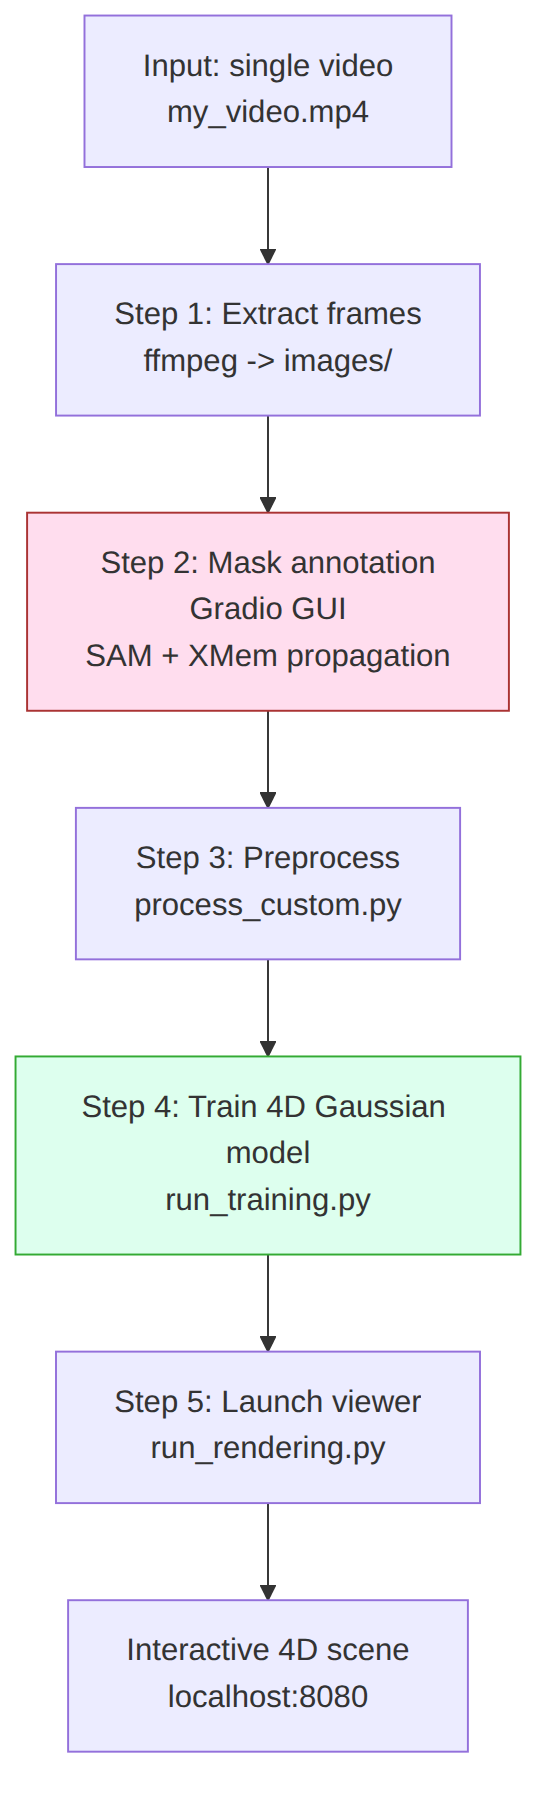
\includegraphics[width=\textwidth,height=0.85\textheight,keepaspectratio]{01_pipeline.png}
  \caption{End-to-end pipeline from input video to interactive 4D viewer.}
\end{figure}

\clearpage
\section{Preprocessing (\texttt{preproc/process\_custom.py})}

Outputs feed the dataloader: per-frame \textbf{RGB + mask + aligned depth +
camera ($K$, $w2c$) + 2D tracks}.

\begin{figure}[H]
  \centering
  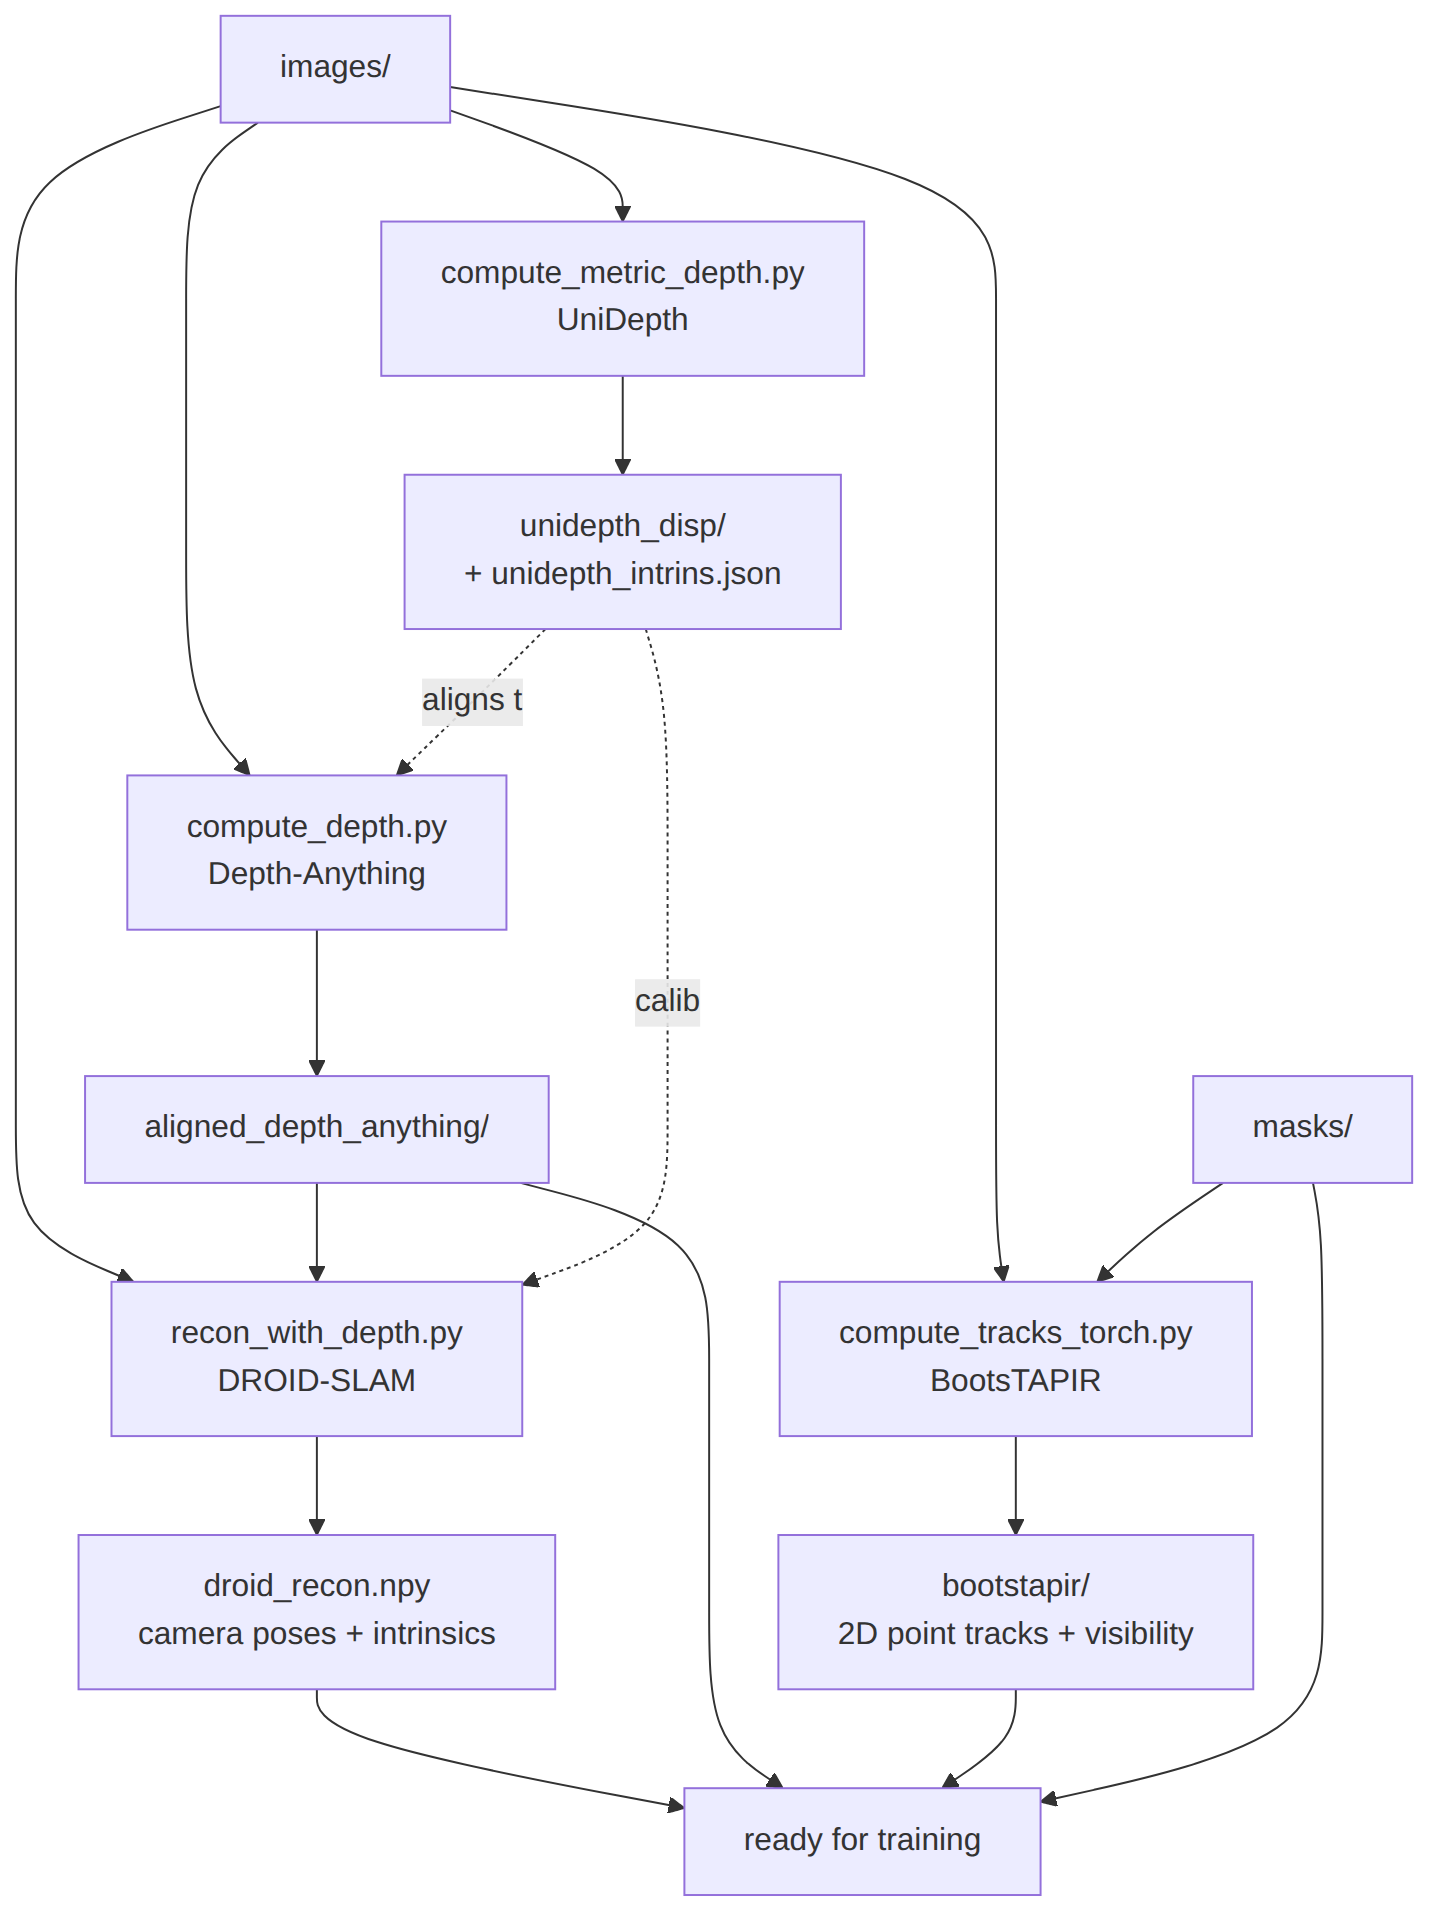
\includegraphics[width=\textwidth,height=0.85\textheight,keepaspectratio]{02_preprocessing.png}
  \caption{Preprocessing pipeline: UniDepth (metric depth), Depth-Anything
  (mono depth, aligned to UniDepth), DROID-SLAM (camera poses), and
  BootsTAPIR (2D tracks).}
\end{figure}

\clearpage
\section{Model initialization (\texttt{init\_model\_from\_tracks} $\rightarrow$ \texttt{SceneModel})}

Key idea: \textbf{foreground motion is parameterized as $K$ shared SE(3)
bases plus per-Gaussian mixing coefficients}, initialized by clustering
track trajectories and solving Procrustes per cluster.

\begin{figure}[H]
  \centering
  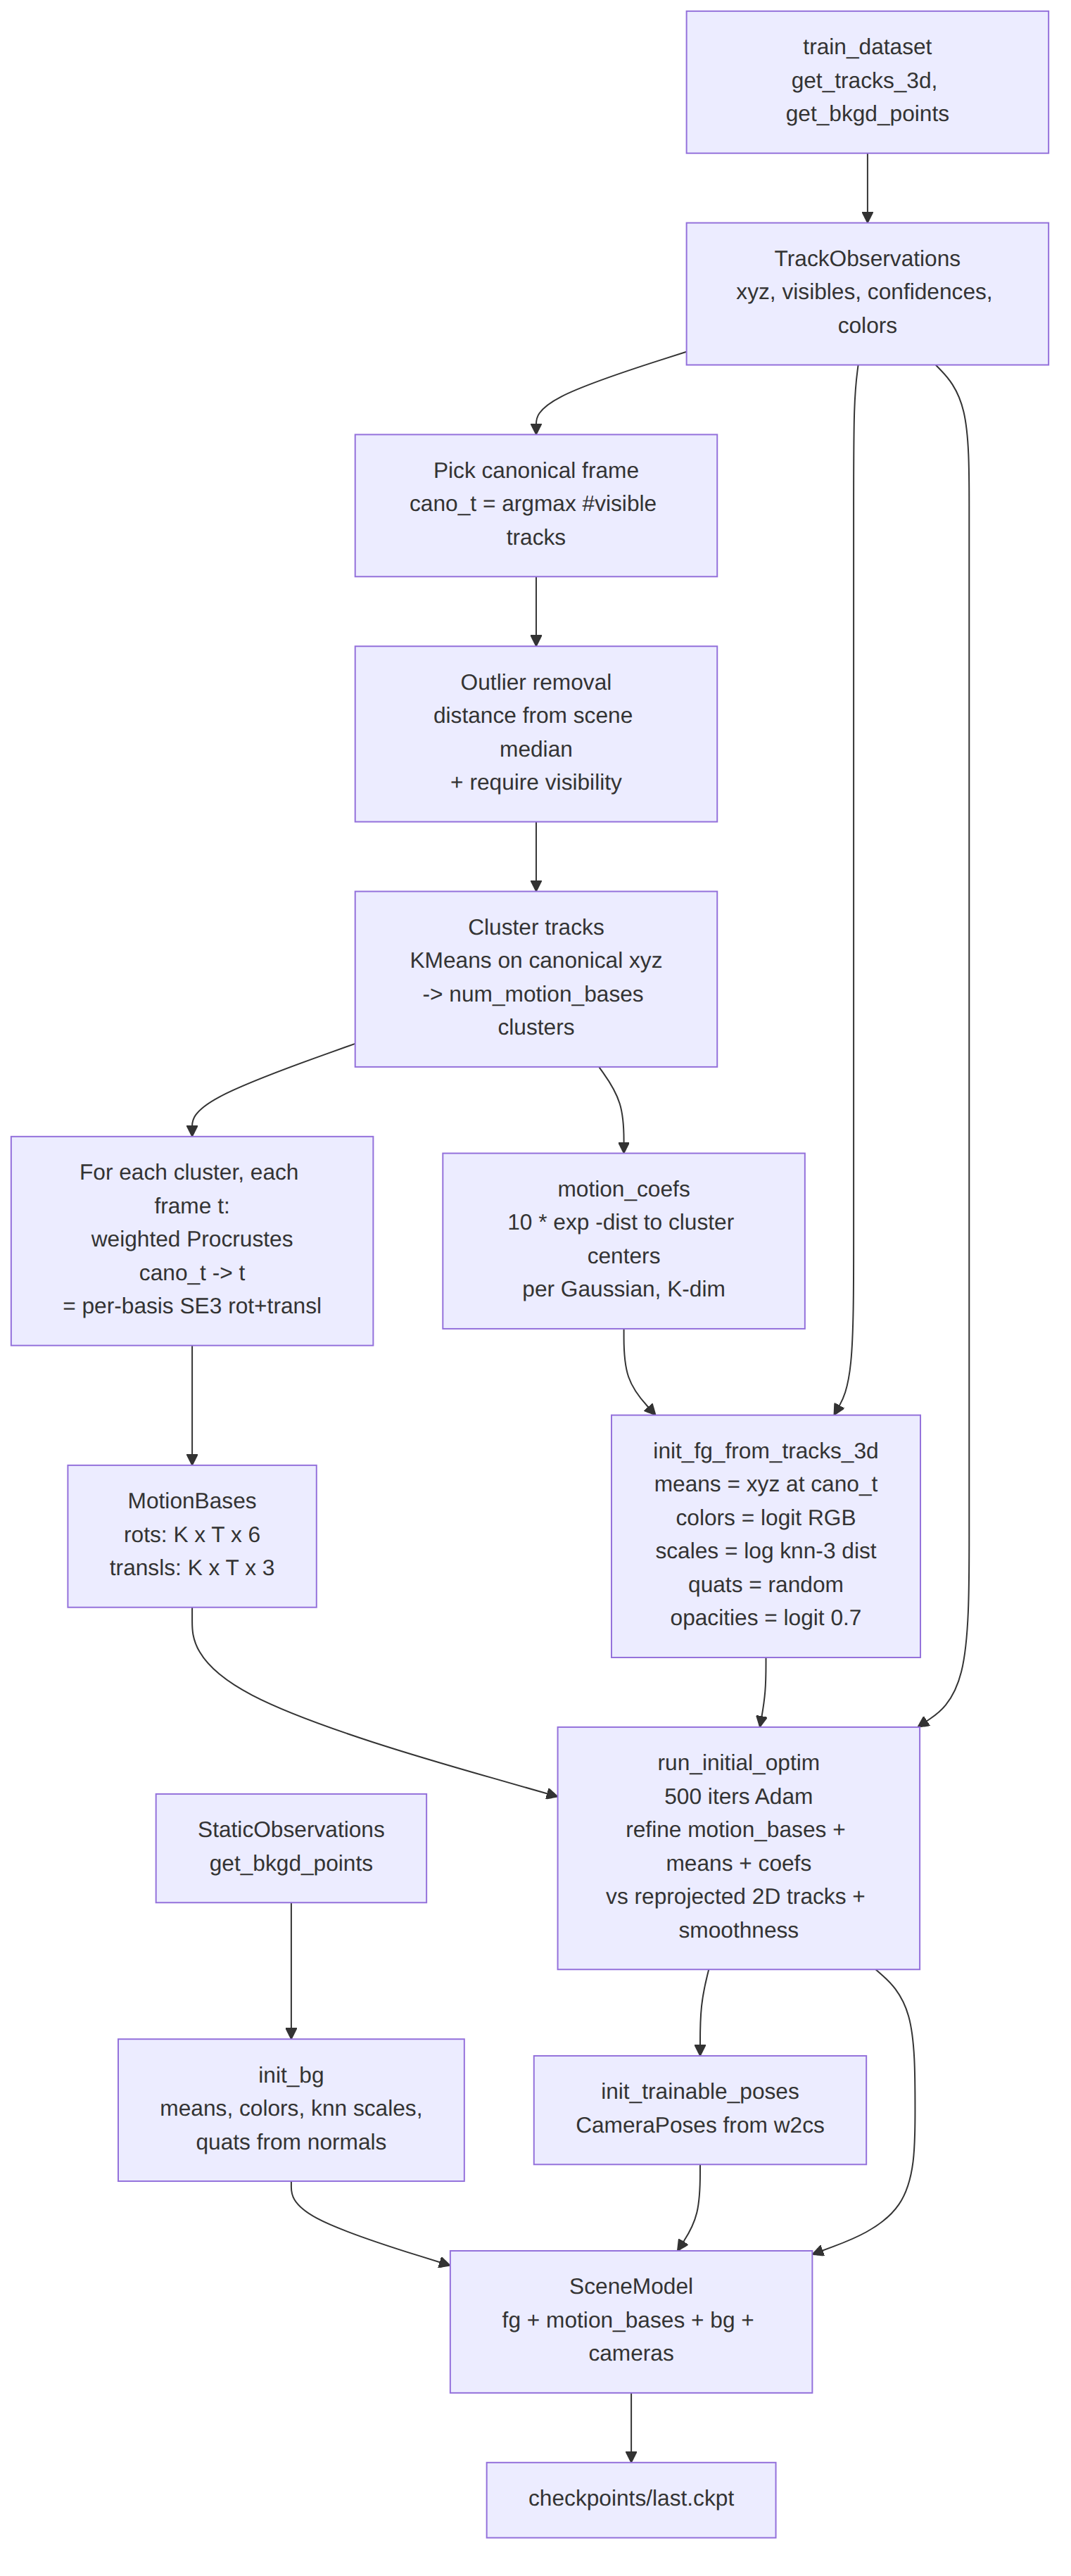
\includegraphics[width=\textwidth,height=0.85\textheight,keepaspectratio]{03_initialization.png}
  \caption{Initialization of foreground Gaussians, motion bases (via weighted
  Procrustes per cluster), background Gaussians, and trainable camera poses.}
\end{figure}

\clearpage
\section{Training loop (\texttt{scripts/run\_training.py} + \texttt{Trainer})}

\begin{figure}[H]
  \centering
  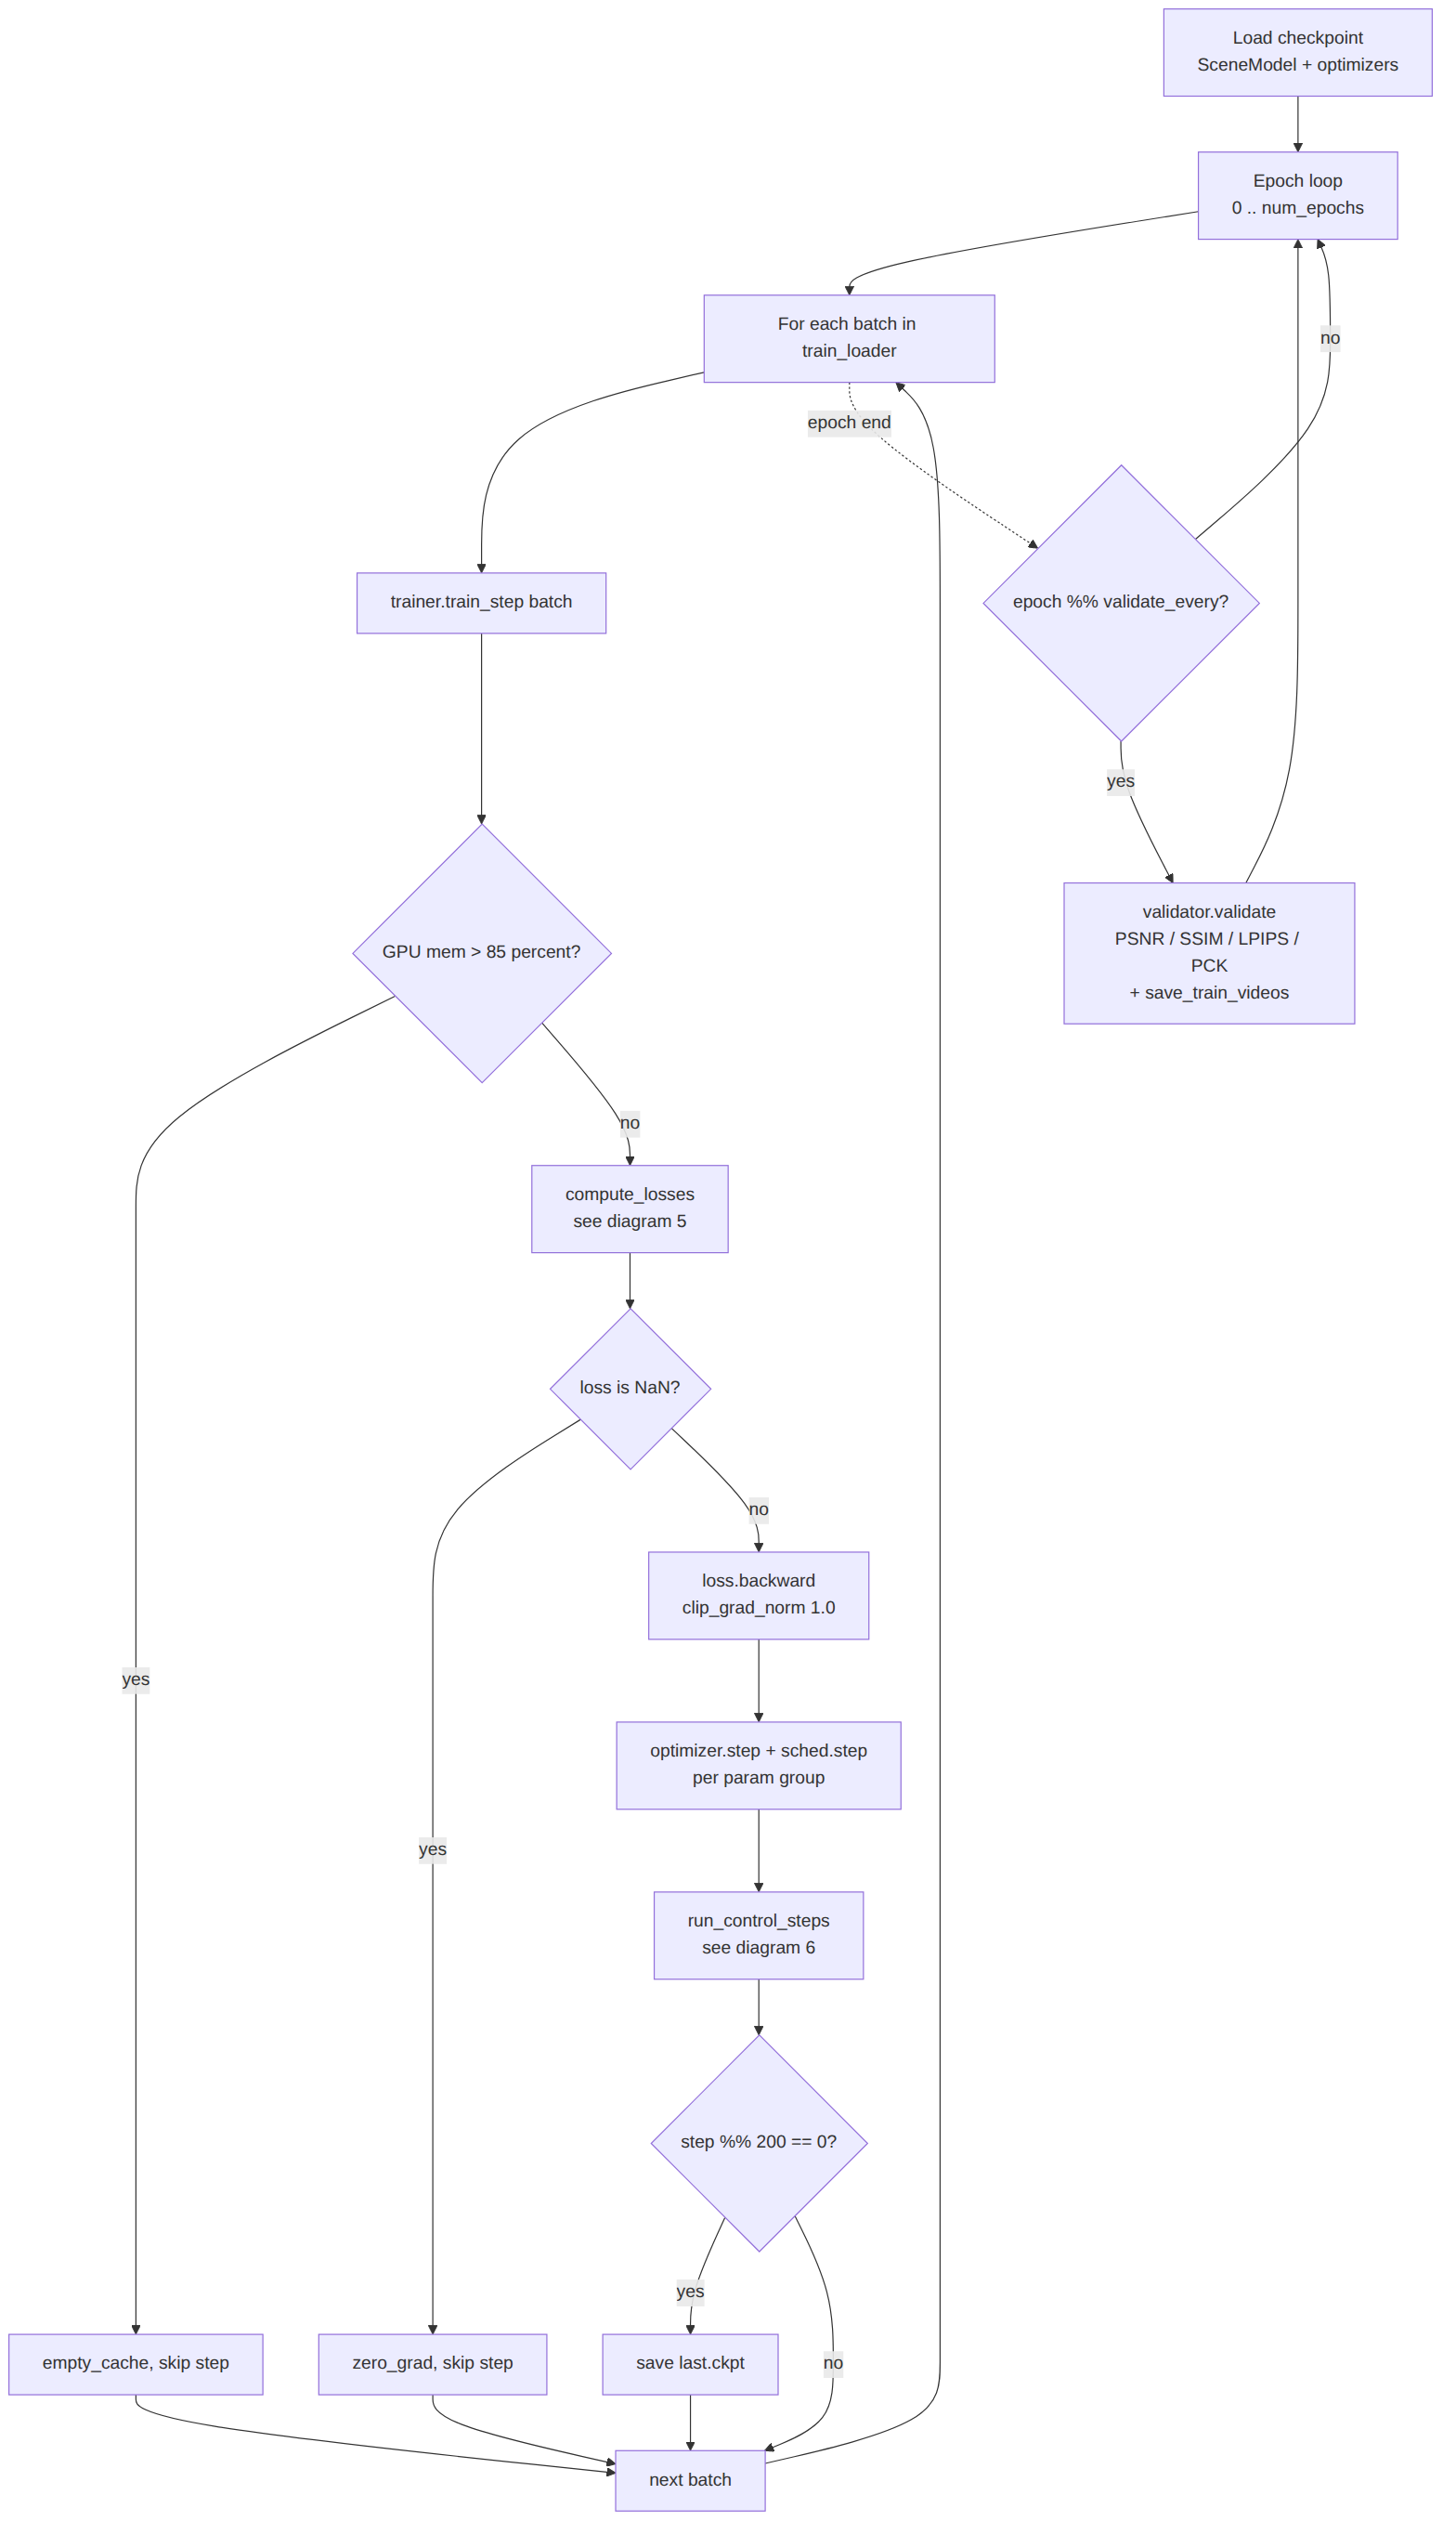
\includegraphics[width=\textwidth,height=0.85\textheight,keepaspectratio]{04_training_loop.png}
  \caption{Outer epoch / batch loop with GPU-memory and NaN guards, gradient
  clipping, periodic checkpointing, and end-of-epoch validation.}
\end{figure}

\clearpage
\section{Per-step loss computation (\texttt{Trainer.compute\_losses})}

\begin{figure}[H]
  \centering
  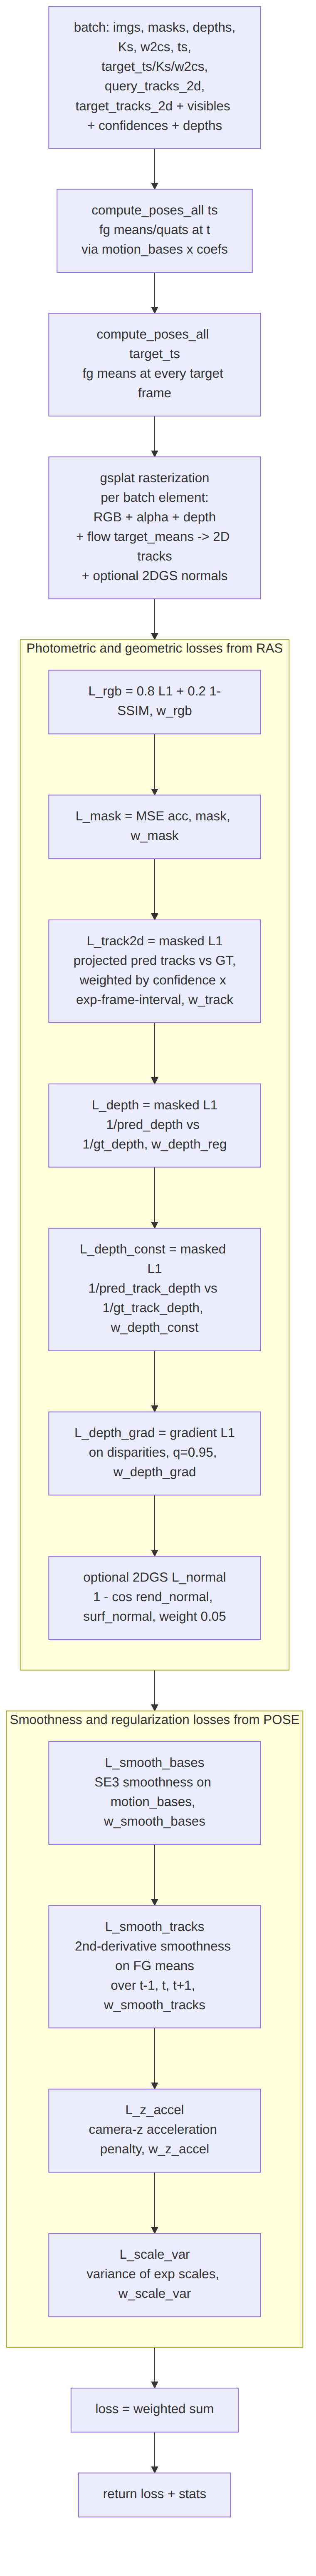
\includegraphics[width=\textwidth,height=0.85\textheight,keepaspectratio]{05_loss_computation.png}
  \caption{All loss terms: photometric (RGB/SSIM), mask, 2D track
  reprojection, depth (disparity / track depth / gradient), optional 2DGS
  normals, and motion smoothness regularizers.}
\end{figure}

\clearpage
\section{Adaptive Gaussian density control (\texttt{run\_control\_steps})}

These three operations (split / duplicate / cull / opacity-reset) keep the
Gaussian count adaptive: dense where the image gradient demands it, sparse
elsewhere.

\begin{figure}[H]
  \centering
  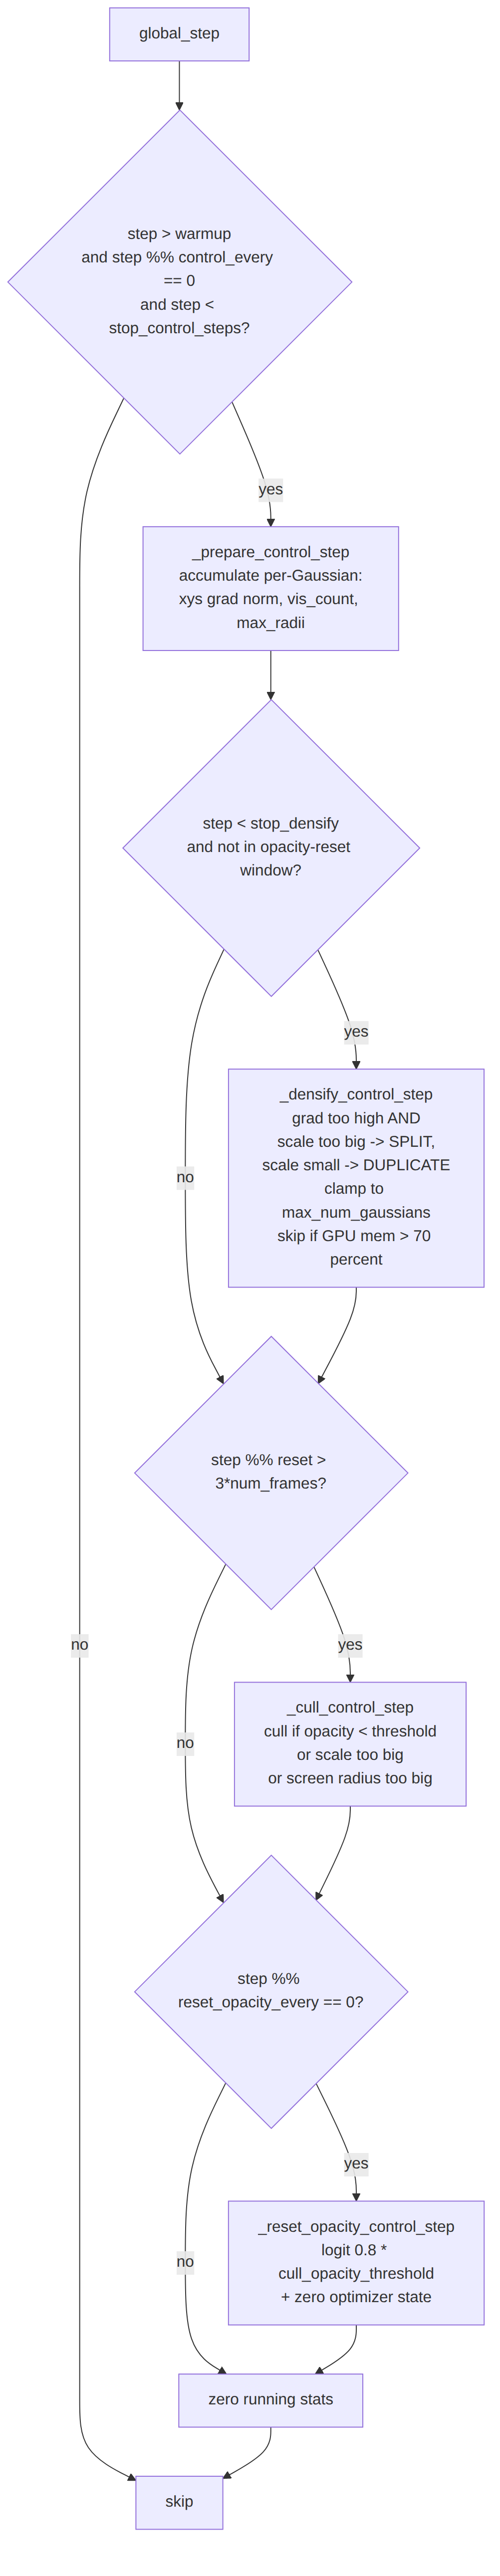
\includegraphics[width=\textwidth,height=0.85\textheight,keepaspectratio]{06_density_control.png}
  \caption{Densify / cull / opacity-reset cycle, gated by warmup, control
  cadence, and GPU memory pressure.}
\end{figure}

\clearpage
\section{SceneModel render path (used in both training and the viewer)}

\begin{figure}[H]
  \centering
  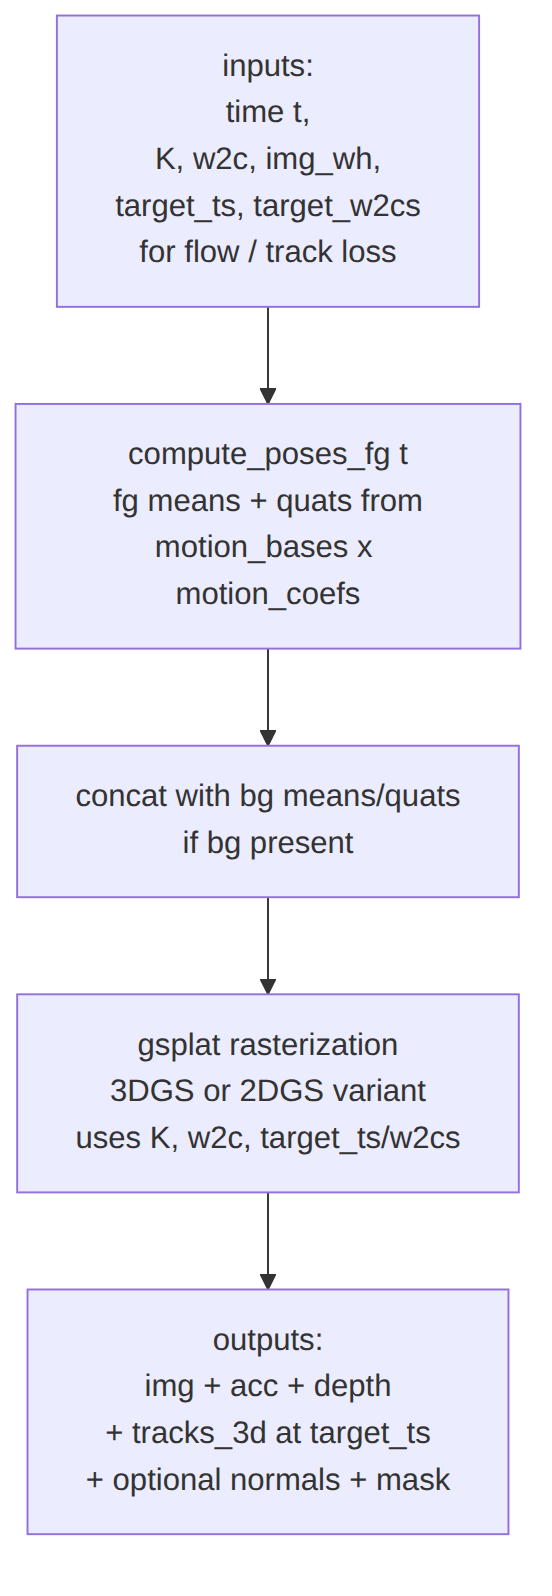
\includegraphics[width=\textwidth,height=0.85\textheight,keepaspectratio]{07_render.png}
  \caption{Render path: time-conditioned foreground poses are computed from
  motion bases $\times$ coefficients, concatenated with static background
  Gaussians, and rasterized via \texttt{gsplat}.}
\end{figure}

\clearpage
\section*{Summary in one sentence}

A single video $\rightarrow$ (depth, camera, 2D tracks, masks) $\rightarrow$
cluster the lifted 3D tracks into $K$ motion bases (Procrustes init)
$\rightarrow$ represent the dynamic foreground as Gaussians whose poses at
any time are mixtures of those $K$ SE(3) bases (plus a static-background
Gaussian splat) $\rightarrow$ optimize via \texttt{gsplat} rasterization
against RGB / mask / depth / 2D-track / smoothness losses, while adaptively
splitting, duplicating, culling, and resetting Gaussians.

\end{document}
